\section{Mathematical Framework}
\label{sec:dag_defs}

To develop our data structure and associated algorithms, we first establish the necessary mathematical definitions and properties concerning weighted DAGs and path weights.

\subsection*{Weighted Directed Acyclic Graphs}
\label{subsec:dag_def}

We begin with the formal definition of the structure central to this chapter.

\begin{definition}[Weighted DAG]
    \label{def:weighted_dag}
    A node-weighted Directed Acyclic Graph (weighted DAG) is a triple $G = (V, E, w)$, where:
    \begin{itemize}
        \item $V$ is a finite set of vertices. We typically identify $V$ with the set $\{0, 1, \dots, n-1\}$ where $n = |V|$, thereby implicitly defining a total order on the vertices.
        \item $E \subseteq V \times V$ is a set of directed edges such that the graph $(V, E)$ contains no directed cycles.
        \item $w: V \to \mathbb{N}_0$ is a weight function assigning a non-negative integer $w(v)$ to each vertex $v \in V$, where $\mathbb{N}_0 = \{0, 1, 2, \dots\}$.
    \end{itemize}
    For a vertex $v \in V$, we denote the set of its direct predecessors as
    \[Pred(v) = \{u \in V \mid (u, v) \in E\}\]
    and the set of its direct successors as
    \[Succ(v) = \{u \in V \mid (v, u) \in E\}.\]
    A vertex $v$ with $Succ(v) = \emptyset$ is termed a sink vertex.
\end{definition}

This definition provides the fundamental object of study. We will often rely on the acyclic property, which guarantees the existence of topological orderings of the vertices.

\begin{assumption}[Unique Source]
    \label{ass:unique_source}
    Without loss of generality, we assume that the DAG $G$ possesses a unique source vertex $s \in V$ characterized by $Pred(s) = \emptyset$. If multiple sources exist in the original graph, a standard preprocessing step involves introducing a virtual source vertex $s'$ with $w(s')=0$ and adding edges $(s', v)$ for all original source vertices $v$. Throughout this work, we assume such a transformation has been applied if necessary, and we identify the unique source with vertex $s=0$, setting $w(s)=0$.
\end{assumption}

Having defined the graph structure, we now define paths and their associated weights, which are central to the queries we aim to support.

\begin{definition}[Path in a DAG]
    \label{def:path}
    A path $P$ from a vertex $u$ to a vertex $v$ in $G$ is a sequence of vertices $P = (v_0, v_1, \dots, v_k)$ such that $v_0 = u$, $v_k = v$, and $(v_{j-1}, v_j) \in E$ for all $1 \le j \le k$. The length of the path $P$ is $k$, the number of edges. Let $Path(s, v)$ denote the set of all paths originating from the unique source $s$ and terminating at $v$.
\end{definition}

\begin{definition}[Cumulative Path Weight]
    \label{def:paths_weights}
    The cumulative weight, denoted $W(P)$, for a path $P=(v_0=s, \dots, v_k=v)$ as defined in \ref{def:path}, is the sum of the weights of the vertices along the path:
    \[ W(P) = \sum_{j=1}^{k} w(v_j). \]
\end{definition}


\subsection{Path Weight Aggregation}
\label{subsec:o_set_def}

A key challenge lies in efficiently representing the potentially vast collection of path weights terminating at each vertex. We introduce a set associated with each vertex to capture precisely this information.

\begin{definition}[$\mathcal{O}$-Set]
    \label{def:o_set}
    For each vertex $v \in V$ in a weighted DAG $G=(V, E, w)$ with source $s$, the $\mathcal{O}$-set, denoted $\mathcal{O}_v \subseteq \mathbb{N}_0$, is defined recursively. Let us assume a topological ordering of the vertices in $V$. The sets are constructed as follows: for the source vertex $v = s$:
    \[ \mathcal{O}_s = \{0\}. \]
    For any other vertex $v \neq s$:
    \[ \mathcal{O}_v = \bigcup_{u \in Pred(v)} \{ y + w(v) \mid y \in \mathcal{O}_u \}. \]
\end{definition}
This definition implies that $\mathcal{O}_v$ contains only the distinct values generated by this union process. We consider $\mathcal{O}_v$ to be the set of these unique values, represented as a sorted sequence.

\begin{figure}[htbp]
    \centering
    % \begin{tikzpicture}[
    %     node distance=1.5cm and 1cm,
    %     base_node/.style={circle, draw=black, thick, minimum size=8mm, inner sep=0pt, font=\sffamily},
    %     root_node/.style={base_node, fill=red!60, text=black},
    %     data_label/.style={font=\tiny\sffamily, text=black},
    %     edge_style/.style={->, >={Stealth[length=2mm]}, thick, draw=black}
    %     ]

    %     \node[root_node, label={[data_label, red, yshift=-0.3cm]below:(0)}] (0) at (0, 2) {0}; % O-set: {0}
    %     \node[base_node, label={[data_label]below:(1)}] (1) at (1.5, 0) {1}; % O-set: {1}
    %     \node[base_node, label={[data_label]above:(3)}] (3) at (1.5, 4) {3}; % O-set: {3}
    %     \node[base_node, label={[data_label]below:(7, 9)}] (6) at (3.5, 1.5) {6}; % O-set: {7, 9}
    %     \node[base_node, label={[data_label]below:(8)}] (7) at (4.5, 0) {7}; % O-set: {8}
    %     % Node 2: O-set {5, 9, 11}
    %     \node[base_node, label={[data_label, xshift=0.3cm]above:(5, 9, 11)}] (2) at (5.5, 4) {2};
    %     % Node 9: O-set {16, 17, 18}
    %     \node[base_node, label={[data_label]above:(16, 17, 18)}] (9) at (6.5, 2) {9};
    %     % Node 5: O-set {13, 21, 22, 23}
    %     \node[base_node, label={[data_label, xshift=0.3cm]below:(13, 21, 22, 23)}] (5) at (9, 0.5) {5};
    %     % Node 10: O-set {15, 19, 21}
    %     \node[base_node, label={[data_label, xshift=0.3cm]above:(15, 19, 21)}] (10) at (8.5, 5) {10};
    %     % Node 8: O-set {21, 23, ..., 31}
    %     \node[base_node, label={[data_label, align=left]right:(21, 23, 24, 25,\\ 26, 27, 29, 30, 31)}] (8) at (11, 3) {8};

    %     \draw [edge_style] (0) -- (1);
    %     \draw [edge_style] (0) -- (3);
    %     \draw [edge_style] (1) -- (6);
    %     \draw [edge_style] (1) -- (7);
    %     \draw [edge_style] (3) -- (2);
    %     \draw [edge_style] (3) -- (6);
    %     \draw [edge_style] (6) -- (2);
    %     \draw [edge_style] (6) -- (9);
    %     \draw [edge_style] (7) -- (5);
    %     \draw [edge_style] (7) -- (9);
    %     \draw [edge_style] (2) -- (10);
    %     \draw [edge_style] (9) -- (5);
    %     \draw [edge_style] (9) -- (8);
    %     \draw [edge_style] (10) -- (8);
    %     \draw [edge_style] (5) -- (8);

    % \end{tikzpicture}
    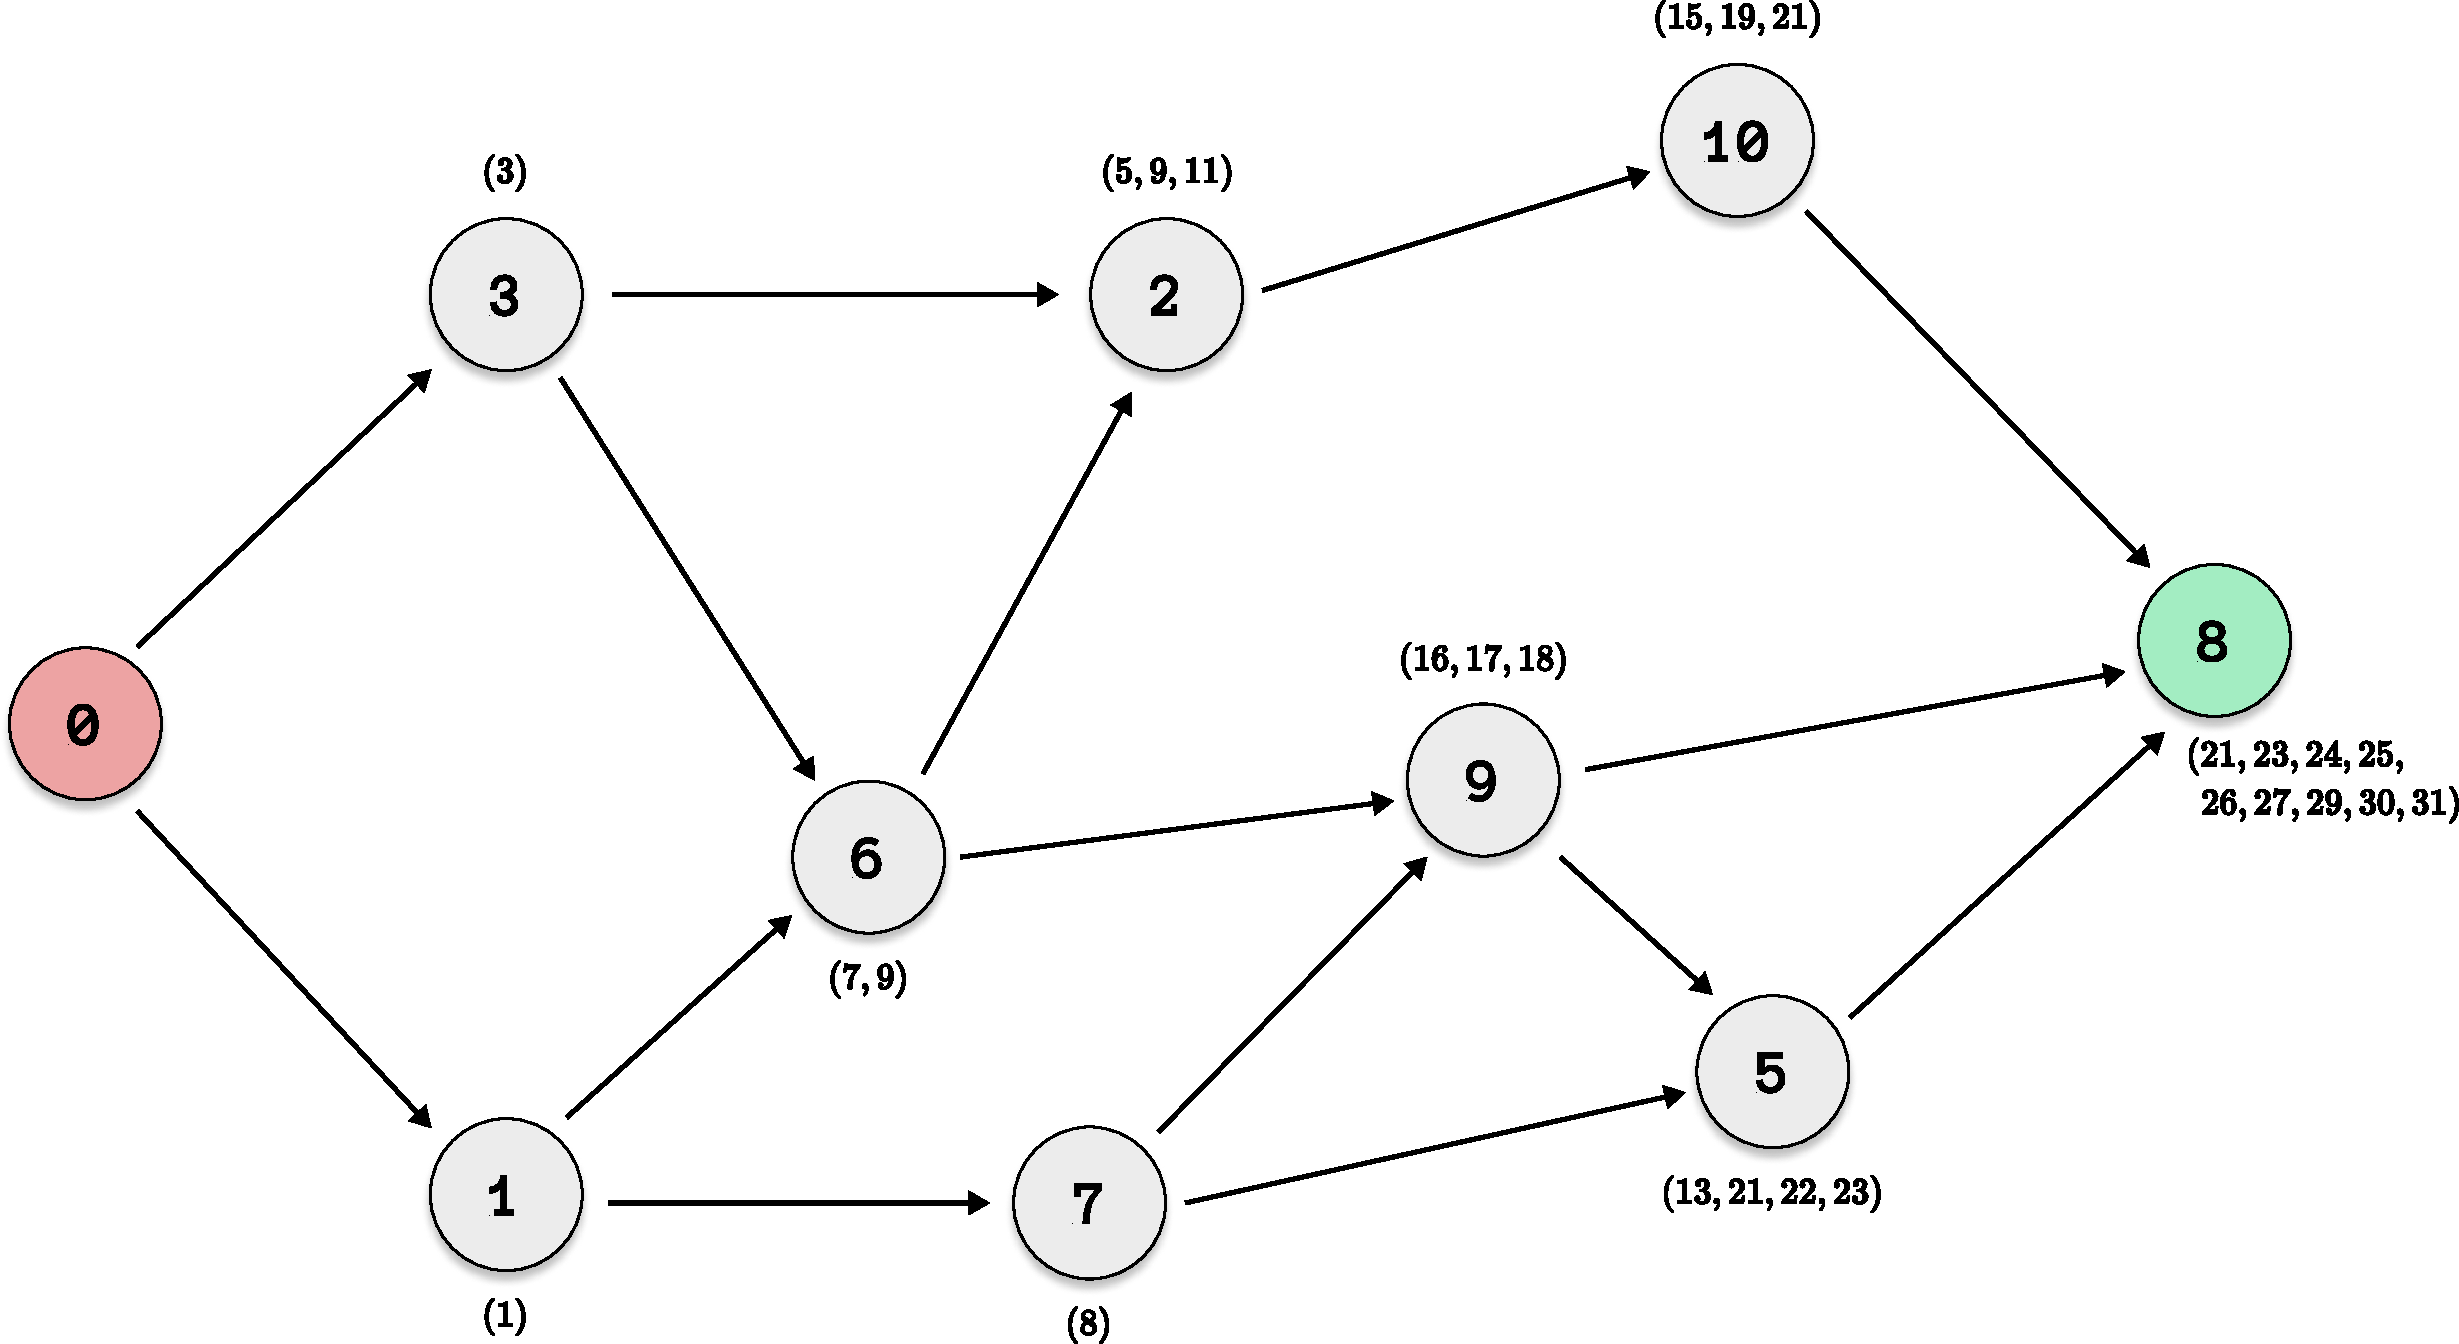
\includegraphics[width=\textwidth]{assets/dag_explicit_final.pdf}
    \caption{Example of a node-weighted DAG. Each node $v$ contains its weight $w(v)$. The label associated with each node represents its calculated $\mathcal{O}$-set, $\mathcal{O}_v$, considered as a sorted sequence.}
    \label{fig:dag_example}
\end{figure}

\begin{example}[$\mathcal{O}$-Set Calculation]
    \label{ex:o_set_calc}
    Consider the weighted DAG shown in \autoref{fig:dag_example}. Each node $v$ is labelled with its weight $w(v)$ inside the circle. The label associated with each node displays its corresponding $\mathcal{O}$-set, calculated according to \ref{def:o_set}.
\end{example}

The following proposition establishes the semantic meaning of the $\mathcal{O}$-set, confirming that it correctly captures the set of all possible path weights (as defined in \ref{def:paths_weights}) ending at a vertex.

\begin{proposition}[Characterization of the $\mathcal{O}$-Set]
    \label{prop:o_set_correctness}
    For any vertex $v \in V$, the set $\mathcal{O}_v$ is equal to the set of cumulative path weights from the source $s$ to $v$:
    \[ \mathcal{O}_v = \{ W(P) \mid P \in Path(s, v) \}. \]
\end{proposition}
\begin{proof}
    The proof proceeds by induction on the vertices $v \in V$, ordered according to a topological sort of $G$.
    \textit{Base Case:} For the source vertex $v=s$, the only path in $Path(s, s)$ is the trivial path $P=(s)$. According to Definition \ref{def:paths_weights}, $W(P)=0$. By Definition \ref{def:o_set}, $\mathcal{O}_s = \{0\}$. Thus, the proposition holds for $s$.
    \textit{Inductive Step:} Assume the proposition holds for all vertices $u$ that strictly precede $v$ in the topological order. In particular, this assumption holds for all $u \in Pred(v)$, since the existence of an edge $(u, v)$ implies $u$ precedes $v$ in any topological sort. We must show that $\mathcal{O}_v = \{ W(P) \mid P \in Path(s, v) \}$.

    ($\subseteq$) Let $x \in \mathcal{O}_v$. By Definition \ref{def:o_set}, since $v \neq s$, there must exist a predecessor $u \in Pred(v)$ and a value $y \in \mathcal{O}_u$ such that $x = y + w(v)$. By the inductive hypothesis applied to $u$, $y = W(P')$ for some path $P' = (v_0=s, \dots, v_{k-1}=u) \in Path(s, u)$. Consider the path $P = (v_0, \dots, v_{k-1}, v_k=v)$ formed by appending the edge $(u, v)$ to $P'$. This is a valid path in $Path(s, v)$. Its weight according to Definition \ref{def:paths_weights} is
    \begin{align*}
        W(P) & = \sum_{j=1}^{k} w(v_j) = \left(\sum_{j=1}^{k-1} w(v_j)\right) + w(v_k) \\
             & = W(P') + w(v) = y + w(v) = x.
    \end{align*}
    Therefore, any element $x \in \mathcal{O}_v$ corresponds to the weight of some path in $Path(s, v)$.

    ($\supseteq$) Let $P = (v_0=s, \dots, v_k=v)$ be an arbitrary path in $Path(s, v)$. Since $v \neq s$, the path must have length $k \ge 1$. Let $u = v_{k-1}$ be the vertex immediately preceding $v$ on this path; thus, $u \in Pred(v)$. Let $P' = (v_0, \dots, v_{k-1})$ be the subpath of $P$ ending at $u$. $P'$ is a path in $Path(s, u)$. By the inductive hypothesis, the weight $W(P') = \sum_{j=1}^{k-1} w(v_j)$ must be an element of $\mathcal{O}_u$. Let $y = W(P')$. By Definition \ref{def:o_set}, the value $y + w(v)$ is included in the construction of $\mathcal{O}_v$. We observe that
    \begin{align*}
        y + w(v) & = W(P') + w(v_k) = \left(\sum_{j=1}^{k-1} w(v_j)\right) + w(v_k) \\
                 & = \sum_{j=1}^{k} w(v_j) = W(P).
    \end{align*}
    Thus, the weight $W(P)$ of any path in $Path(s, v)$ is contained in $\mathcal{O}_v$.

    Since both inclusions hold, we conclude that $\mathcal{O}_v = \{ W(P) \mid P \in Path(s, v) \}$.
\end{proof}

An important property related to the sizes of these $\mathcal{O}$-sets is monotonicity along edges, which plays a fundamental role in the design of our succinct structure.

\begin{lemma}[$\mathcal{O}$-Set Cardinality Monotonicity along Edges]
    \label{lem:o_set_cardinality_monotonicity}
    Let $v \in V$ and let $u \in Succ(v)$ be any direct successor of $v$. Then, the cardinality of the $\mathcal{O}$-set of $v$ is less than or equal to the cardinality of the $\mathcal{O}$-set of $u$, i.e., $|\mathcal{O}_v| \le |\mathcal{O}_u|$.
\end{lemma}
\begin{proof}
    From Definition \ref{def:o_set}, the $\mathcal{O}$-set for $u$ is given by
    \[ \mathcal{O}_u = \bigcup_{p \in Pred(u)} \{ y + w(u) \mid y \in \mathcal{O}_p \}. \]
    Since $u$ is a successor of $v$, it follows that $v$ is a predecessor of $u$, i.e., $v \in Pred(u)$. Therefore, the set $S_v = \{ y + w(u) \mid y \in \mathcal{O}_v \}$ contributes to the union forming $\mathcal{O}_u$. Specifically
    \[S_v \subseteq \bigcup_{p \in Pred(u)} \{ y + w(u) \mid y \in \mathcal{O}_p \}\]
    Consider the mapping $f: \mathcal{O}_v \to S_v$ defined by $f(y) = y + w(u)$. Since $w(u) \ge 0$, this mapping is injective. If $y_1 \neq y_2$, then $y_1 + w(u) \neq y_2 + w(u)$. Consequently, the number of distinct elements in $S_v$ is exactly equal to the number of distinct elements in $\mathcal{O}_v$, so $|S_v| = |\mathcal{O}_v|$.
    The set $\mathcal{O}_u$ is formed by taking the union of sets like $S_v$ for all predecessors $p \in Pred(u)$ and retaining only the unique values. Since the elements generated from $v$'s contribution (namely, $S_v$) are a subset of the elements considered for $\mathcal{O}_u$, the total number of unique elements in $\mathcal{O}_u$ must be at least the number of unique elements contributed by $v$.
    Therefore, $|\mathcal{O}_u| \ge |S_v| = |\mathcal{O}_v|$.
\end{proof}



\subsection{The Rank Query}
\label{subsec:rank_dag_def}

Having defined the $\mathcal{O}$-set, which precisely captures the set of all possible cumulative path weights terminating at a given vertex $N$, we now introduce the \textsf{rank} query. This query builds upon the $\mathcal{O}$-set to provide a richer description related to the path weights.

Intuitively, each value $x \in \mathcal{O}_N$ represents the total accumulated weight along some path from the source $s$ ending exactly at $N$. We can think of the weight $w(N)$ of the node $N$ itself as the contribution or cost associated with the final step or "activity" performed at $N$. The \textsf{rank} query, $\mathrm{rank}_G(N)$, aims to capture not just the final cumulative weights $x \in \mathcal{O}_N$, but rather the set of all possible cumulative values that could be considered "active" or relevant \emph{during} the activity represented by node $N$.

Specifically, for a path $P$ reaching $N$ with total weight $W(P)=x$, the query considers the range of cumulative values from the point just before incorporating $N$'s full weight up to the final value $x$. This corresponds mathematically to the integer interval
\[[\max(0, x - w(N) + 1), x]\]
This interval represents all possible integer cumulative weights observed during the \emph{processing} of node $N$ along that specific path. The \textsf{rank} query then aggregates these intervals over all possible paths ending at $N$.

This intuition leads to the following formal definition:

\begin{definition}[Rank Query on Weighted DAG]
    \label{def:rank_dag}
    Given a vertex $N \in V$ in a weighted DAG $G=(V, E, w)$, the rank query, denoted $\mathrm{rank}_G(N)$, returns a representation of a specific set of integers derived from the $\mathcal{O}$-set $\mathcal{O}_N$. The target set, $S_N \subseteq \mathbb{N}_0$, is defined as the union of intervals generated from each element $x \in \mathcal{O}_N$:
    \[ S_N = \bigcup_{x \in \mathcal{O}_N} \{ z \in \mathbb{N}_0 \mid \max(0, x - w(N) + 1) \le z \le x \}. \]
    These intervals are then maximally merged, meaning $r_k < l_{k+1}-1$ for all $k=1, \dots, p-1$. The query result is specified as a minimal collection of disjoint, closed integer intervals,
    \[ \mathcal{R}_N = \{[l_1, r_1], [l_2, r_2], \dots, [l_p, r_p]\} \]
    such that their union exactly covers $S_N$,
    \[ \bigcup_{k=1}^{p} [l_k, r_k] = S_N \]
\end{definition}

% \begin{remark}
%     As motivated above, the transformation from $\mathcal{O}_N$ to the set $S_N$ via the interval generation rule $\{ z \mid \max(0, x - w(N) + 1) \le z \le x \}$ formalizes the idea of capturing the range of values associated with the final node $N$ for each possible incoming path weight $x$. The length of the generated interval is typically $w(N)$ (unless $x < w(N)-1$, in which case it starts from 0), ending precisely at $x$. This mathematical formulation directly implements the intuition of considering values accumulated during the phase associated with node $N$. The subsequent union and merging into disjoint intervals provide a canonical and compact representation of the overall set $S_N$.
% \end{remark}


\begin{example}[Rank Query Calculation]
    \label{ex:rank_calc_disjoint}
    Let us compute the rank query for vertex $N=2$ in the DAG shown\footnote{In this example, the weight function $w$ assigns to each vertex $v$ a weight equal to its identifier, i.e., $w(v)=v$. This is possible since it's just a small graph and we have taken unique weights} in \autoref{fig:dag_example}. From Example \ref{ex:o_set_calc}, we know that the weight of node 2 is $w(2) = 2$, and its $\mathcal{O}$-set is $\mathcal{O}_2 = \{ 5, 9, 11 \}$. These are the possible total weights of paths ending at node 2.
    Applying Definition \ref{def:rank_dag}, we associate an interval with each $x \in \mathcal{O}_2$, representing the values active during the processing of node 2:
    \begin{itemize}
        \item For path weight $x=5$: Interval is $[\max(0, 5 - 2 + 1), 5] = [4, 5]$. These are the values active while accumulating the weight $w(2)=2$ to reach 5.
        \item For path weight $x=9$: Interval is $[\max(0, 9 - 2 + 1), 9] = [8, 9]$.
        \item For path weight $x=11$: Interval is $[\max(0, 11 - 2 + 1), 11] = [10, 11]$.
    \end{itemize}
    The target set $S_2$ is the union of these intervals: $S_2 = [4, 5] \cup [8, 9] \cup [10, 11]$.
    We merge these intervals to obtain the minimal disjoint representation $\mathcal{R}_2$.
    \begin{itemize}
        \item Compare $[4, 5]$ and $[8, 9]$. Since $8 > 5 + 1$, they remain separate.
        \item Compare $[8, 9]$ and $[10, 11]$. Since $10 \le 9 + 1$, they are merged into $[8, \max(9, 11)] = [8, 11]$.
    \end{itemize}
    The final minimal collection of disjoint intervals is:
    \[ \mathrm{Rank}_G(2) = \{ [4, 5], [8, 11] \}. \]
    This collection represents the set $S_2 = \{4, 5\} \cup \{8, 9, 10, 11\}$, which encompasses all possible integer cumulative weights that could be considered active during the processing phase associated with node 2, across all possible paths leading to it.
\end{example}
